\section{System Design}

\subsection{System Architecture}

\begin{figure}[!h]
    \centering
    \includegraphics[width=3.4in]{sysarch.jpeg}
    \caption{System Architecture.}
    \label{fig:sysarch}
\end{figure}

\subsubsection{Energy Harvesting and Voltage Conditioning} 
This represents an energy harvesting front end that can gain power from environmental sources and condition that to be able to power the rest of the system. 
One requirement is that this module should be able to provide current when $0 < V_{cc} < V_{calibrate}$.

\subsubsection{Capacitor} 
In intermittently-powered systems, the harvested energy is then buffered in a capacitor, typically in a \SI{}{\micro\farad} to \SI{}{\milli\farad} scale. 

\subsubsection{Microcontroller}
The MCU is enabled to execute intermittently. It also controls a switch to disconnect or connect the supply during calibration. 
The switch is normally open, but can be closed during calibration. 

\subsubsection{Voltage Monitor}
This module monitors $V_{cc}$ and signals the MCU to wake up or sleep. 
The monitored voltage thresholds can be set by the MCU. 
This can be an external low-power component or an internal comparator of the MCU. 

\subsection{Online Task Calibration}

\begin{figure}[!h]
    \centering
    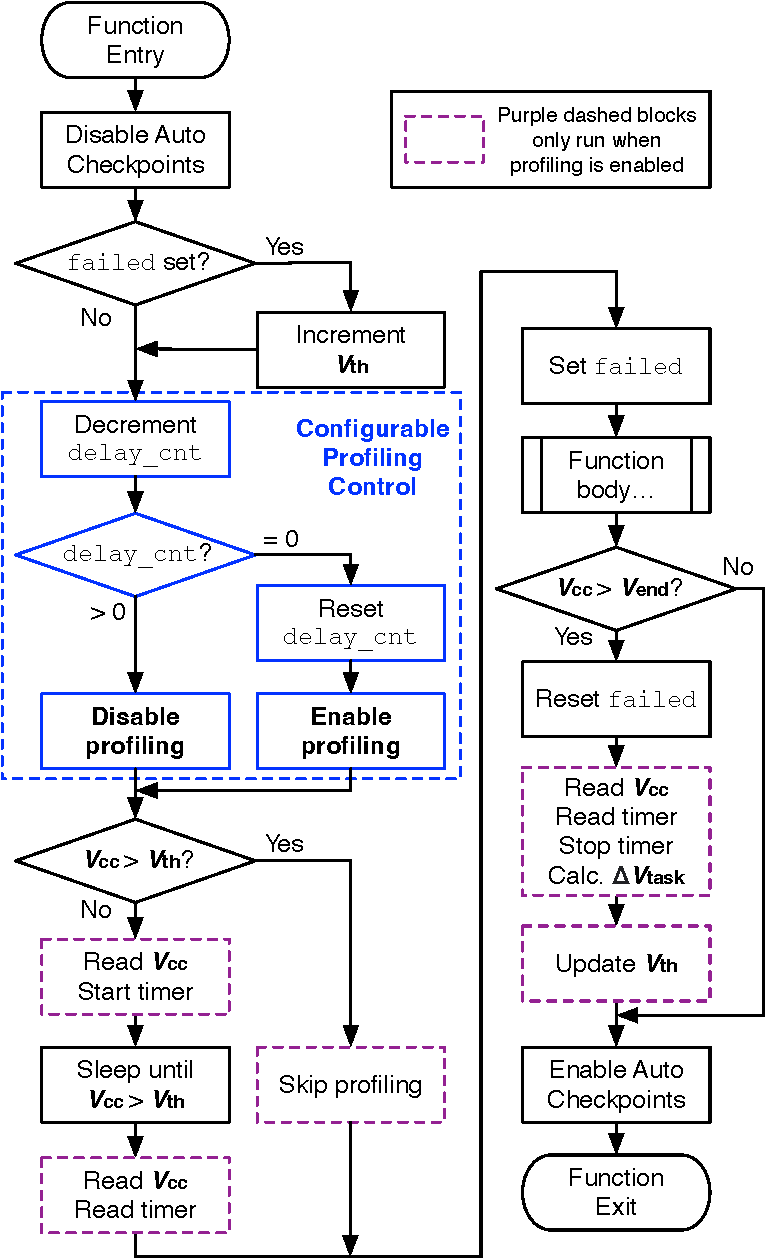
\includegraphics[width=3in]{flowchart.pdf}
    \caption{Flowchart.}
    \label{fig:flowchart}
\end{figure}

The programmers are able to denote separate atomic tasks. 
The handling routine for each task is shown in \figurename{~\ref{fig:flowchart}}. 

When to calibrate? 
When the denoted task is executed, the routine switches to calibration if the atomic segment fails in the last execution or is not calibrated. 
Execution failure is checked by setting and resetting a nonvolatile variable when the atomic segment begins and finishes.

How to define $V_{calibrate}$? 
Align this to the smaller one between the maximum operating voltage and the highest $V_{cc}$ that the energy harvesting can output. 

\subsection{Threshold Adaptation}

The calibration process measures the voltage drop of purely executing an atomic task. It is a question how to translate this voltage drop to a corresponding threshold. 

An assumption is the atomic tasks consume approximately constant current rather than constant power. This needs validation. If they consume constant power, the conversion needs more maths. 

\begin{equation}
    V_{th} = Roundup(V_{drop} + V_{min})
    \label{eq:vth}
\end{equation}

\subsubsection{Constant Model}

In this case, the conversion would be simply:
\begin{equation}
    V_{drop} = C
\end{equation}


\subsubsection{Linear Model}

For workloads where overheads being linear to an input, calibration needs to be performed twice. 
\begin{equation}
    V_{drop} = Ax + C
\end{equation}
